\section{Podstawy teoretyczne} 
Przed omówieniem tematu naszej pracy, należy przedstawić kilka pojęć z teorii grafów, bez których zrozumienia, nie jest możliwe wyznaczanie liczb Ramseya.

  \subsection{Teoria grafów}
  \begin{definition}
    Graf nieskierowany to para G=(V, E), gdzie V to zbiór elementów nazywanych wierzchołkami a E to zbiór par wierzchołków, którego elementy są nazywane krawędziami.
  \end{definition}

  Dla potrzeb naszej pracy, będziemy zakładać, że gdy mówimy o grafie, mamy na myśli graf nieskierowany i prosty (brak duplikatów par w zbiorze E).
  
  \begin{definition}
    Liczbę elementów zbioru V w grafie G=(V, E) nazywamy rzędem grafu. 
  \end{definition}

  Rząd grafu to liczba jego wierzchołków. 

  \begin{definition}
    W grafie G (V, E) wierzchołki u, v $\in$ V sąsiadują wtedy i tylko wtedy gdy (u, v) $\in$ E.    
  \end{definition}
  W grafach nieskierowanych sąsiedztwo jest relacją symetryczną. Jest nieprzechodnia - z sąsiedztwa u i v oraz v i w nie wynika sąsiedztwo u i w. \linebreak

  \begin{figure}[h]
    \centering
    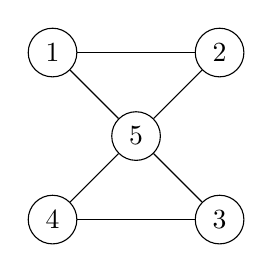
\begin{tikzpicture}[node distance={15mm}, main/.style = {draw, circle}] 
      \node[main] (1) {$1$};
      \node[main] (2) [below right of=1] {$5$};
      \node[main] (3) [above right of=2] {$2$};
      \node[main] (4) [below left of=2] {$4$};
      \node[main] (5) [below right of=2] {$3$};

      \draw (1) -- (2);
      \draw (2) -- (3);
      \draw (2) -- (4);
      \draw (2) -- (5);
      \draw (1) -- (3);
      \draw (4) -- (5);
    \end{tikzpicture}
    \caption{Graf, w którym wierzchołek 1 sąsiaduje z 2 i 5; 2 z 1 i 5; 3 z 4 i 5; 4 z 3 i 5; 5 z 1, 2, 3 i 4 }
  \end{figure}

   \begin{definition}
    Klika $K$ w grafie $G(V,E)$ jest takim podzbiorem wierzchołków $V(G)$, że dla każdej pary wierzchołków $$u, v \in K, (u, v) \in E(G)$$ 
   \end{definition}
   
   W uproszczeniu, klika to podzbiór wierzchołków grafu, z których każdy jest połaczony z każdem innym wiechołkiem tego podzbioru.
   \begin{figure}[H]
   \centering
    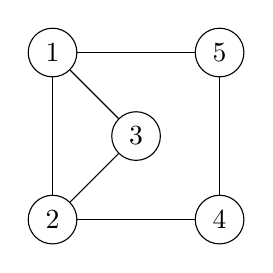
\begin{tikzpicture}[node distance={15mm}, main/.style = {draw, circle}] 
      \node[main] (1) {$1$};
      \node[main] (3) [below right of=1] {$3$};
      \node[main] (2) [below left of=3] {$2$};
      \node[main] (4) [below right of=3] {$4$};
      \node[main] (5) [above right of=3] {$5$};
      
      \draw (3) -- (2);
      \draw (1) -- (3);
      \draw (1) -- (2);
      \draw (2) -- (4);
      \draw (4) -- (5);
      \draw (1) -- (5);
     \end{tikzpicture}
     \caption{Wierzchołki 1, 2, 3 tworzą klikę stopnia 3 - $K_3$ }
  \end{figure}

  Znalezienie stopnia maksymalnej kliki w danym grafie jest trudne obliczeniowo.
  W ogólności jest to problem rozwiązywany w czasie niewielomianowym (chociaż dla niektórych grup grafów, 
  takich jak grafy planarne, istnieją algorytmy wielomianowe), ale sprawdzenie czy w grafie istnieje klika
  z góry znanego stopnia, jest łatwe. Przykładowo istnienie $K_3$ możemy sprawdzić następującym algorytmem:
  
  \begin{algorithm}
    \caption{Sprawdzenie czy graf zawiera $K_3$}
    \begin{algorithmic}
    \REQUIRE $G(V, E) $
    \FORALL{$v in V$}
      \FORALL{$u in V$}
        \IF{$v \neq u \land v \in sasiedzi(u) \land sasiedzi(v) \cap sasiedzi(u) \neq \emptyset$}
          \STATE \RETURN jest $K3$
        \ENDIF
      \ENDFOR
    \ENDFOR
    \STATE \RETURN nie ma K3
    \end{algorithmic}
  \end{algorithm}

  \begin{definition}
    Zbiór niezależny $N$ w grafie $G(V,E)$ to taki podzbiór wierzchołków G, że dla każdej pary wierzchołków $$u, v \in N, (u, v) \notin E(V) $$. 
  \end{definition}

    \begin{figure}[H]
      \centering
       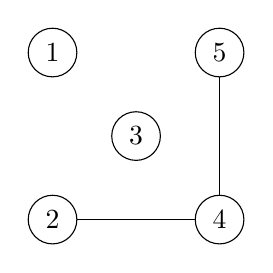
\begin{tikzpicture}[node distance={15mm}, main/.style = {draw, circle}] 
         \node[main] (1) {$1$};
         \node[main] (3) [below right of=1] {$3$};
         \node[main] (2) [below left of=3] {$2$};
         \node[main] (4) [below right of=3] {$4$};
         \node[main] (5) [above right of=3] {$5$};

         \draw (2) -- (4);
         \draw (4) -- (5);

        \end{tikzpicture}
        \caption{Wierzchołki 1, 2, 3, 5 tworzą zbiór niezależny 4 - $N_4$ }
     \end{figure}


     Zbiór niezależny można również zdefiniować jako przeciwieństwo kliki, lub jako klikę w dopełnieniu grafu.

    \begin{definition}
      Depełnieniem grafu $G(V,E)$ nazywamy taki graf $G'(V,E')$, 
      dla którego zachodzi 
      $$\forall{u,v} (u,v) \in E \iff (u,v) \notin E'$$
    \end{definition}
  
    \begin{figure}[H]
      \centering
       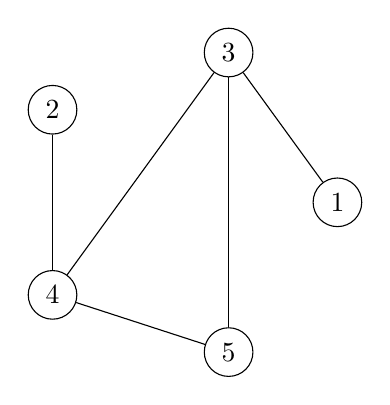
\begin{tikzpicture}[node distance={15mm}, main/.style = {draw, circle}] 
        \node[main] (1) at (0:2){$1$};
        \node[main] (3) at (72:2) {$3$};
        \node[main] (2) at (144:2) {$2$};
        \node[main] (4) at (216:2) {$4$};
        \node[main] (5) at (288:2) {$5$};

         \draw (1) -- (3);
         \draw (2) -- (4);
         \draw (3) -- (5);
         \draw (3) -- (4);
         \draw (4) -- (5);

        \end{tikzpicture}
        \caption{Graf G }
     \end{figure}

     Na pierwszy rzut oka trudno zauważyć czy graf $G$ posiada zbiór niezależny $N_3$.
     Spójrzmy na jego dopełnienie:

     \begin{figure}[H]
      \centering
       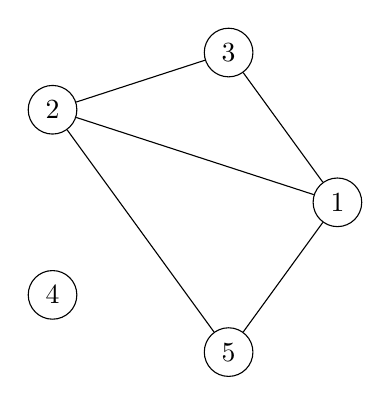
\begin{tikzpicture}[node distance={15mm}, main/.style = {draw, circle}] 
         \node[main] (1) at (0:2){$1$};
         \node[main] (3) at (72:2) {$3$};
         \node[main] (2) at (144:2) {$2$};
         \node[main] (4) at (216:2) {$4$};
         \node[main] (5) at (288:2) {$5$};

         \draw (1) -- (2);
         \draw (1) -- (3);
         \draw (1) -- (5);
         \draw (2) -- (3);
         \draw (2) -- (5);

        \end{tikzpicture}
        \caption{ Dopełnienie grafu G - graf G' }
     \end{figure}

     Natychmiast zauważamy, że graf $G'$ posiada klikę $K_3$:
    Oznacza to, że $G$ ma $N_3$ na tych samych Wierzchołkach.

    \begin{figure}[H]
      \centering
       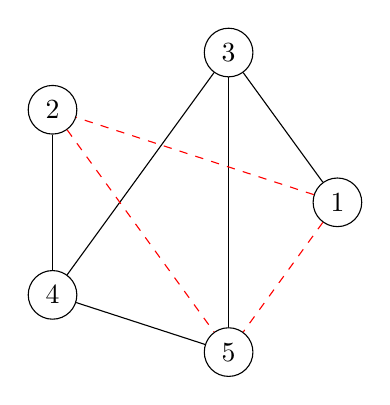
\begin{tikzpicture}[node distance={15mm}, main/.style = {draw, circle}] 
        \node[main] (1) at (0:2){$1$};
        \node[main] (3) at (72:2) {$3$};
        \node[main] (2) at (144:2) {$2$};
        \node[main] (4) at (216:2) {$4$};
        \node[main] (5) at (288:2) {$5$};

         \draw (1) -- (3);
         \draw (2) -- (4);
         \draw (3) -- (5);
         \draw (3) -- (4);
         \draw (4) -- (5);

         \draw[red, dashed] (1) -- (2);
         \draw[red, dashed] (1) -- (5);
         \draw[red, dashed] (2) -- (5);

        \end{tikzpicture}
        \hspace{15mm}
       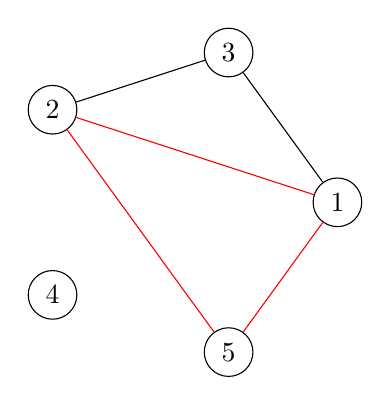
\begin{tikzpicture}[node distance={15mm}, main/.style = {draw, circle}] 
         \node[main] (1) at (0:2){$1$};
         \node[main] (3) at (72:2) {$3$};
         \node[main] (2) at (144:2) {$2$};
         \node[main] (4) at (216:2) {$4$};
         \node[main] (5) at (288:2) {$5$};

         \draw[red] (1) -- (2);
         \draw (1) -- (3);
         \draw[red] (1) -- (5);
         \draw (2) -- (3);
         \draw[red] (2) -- (5);

        \end{tikzpicture}
        \caption{ $K_3$ w $G'$ leży między tymi samymi Wierzchołkami co $N_3$ w $G$ }
     \end{figure}


     \begin{definition}
       Dla grafu $G(V,E)$ i podzbioru jego wierzchołków $S \subseteq V$, 
       podgrafem indukowanym G[S] nazywamy taki graf, którego wszystkie wierzchołki
       zawierają się w S i którego zbiór krawędzi zawiera wszystkie krawędzie z E kończące się w S.
       $$ G[S] = H(S, E_2), \forall (v,u) \in E, (v,u) \ in E_2 \iff v \in S \land u \in S$$ 
     \end{definition}


  \subsection{Izomorfizm}

  \begin{definition}
    Izomorfizm grafów G i H to taka biekcja f:V(G) -> V(H), że 2 wierchołki u i v sąsiadują w G tylko jeżeli f(u) i f(v) sąsiadują w H.
  \end{definition}

  Innymi słowy, izomorfizm jest to takie przekształcenie grafu, które zachowuje wszystkie jego właściwości. Grafy, dla których można znaleźć izomorfizm są izomorficzne. Innymi słowy, dwa grafy są izomorficzne, jeżeli ich wierzchołki można nazwać w taki sposób, 
  aby sąsiadami odpowiadających sobie wierzchołków w obu grafach miały dokładnie takie same zbiory sąsiadów.
  

  Przekształćmy graf z rysunku 1 zamieniając wierzchołek 1 z 2 oraz 3 z 4:
  \begin{figure}[H]
    \centering
    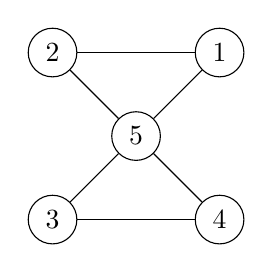
\begin{tikzpicture}[node distance={15mm}, main/.style = {draw, circle}] 
      \node[main] (1) {$2$};
      \node[main] (2) [below right of=1] {$5$};
      \node[main] (3) [above right of=2] {$1$};
      \node[main] (4) [below left of=2] {$3$};
      \node[main] (5) [below right of=2] {$4$};

      \draw (1) -- (2);
      \draw (2) -- (3);
      \draw (2) -- (4);
      \draw (2) -- (5);
      \draw (1) -- (3);
      \draw (4) -- (5);
    \end{tikzpicture}
    \caption{Mimo przekształcenia graf zachował swoje własności}
  \end{figure}

  Jak widać, wierzchołki o tych samych numerach zachowały swoje zbiory sąsiadów. 

  Warto zauważyć, że na nasz użytek grafy izomorficzne nie są niezależnie użyteczne. Wszystkie własności opisane w tej pracy są przez izomorfizmy niezmienione, a więc na nasz użytek dwa grafy izomorficzne to efektywnie ten sam graf.


  \begin{definition}
    Automorfizm grafu G to taka permutacja f zbioru wierzchołków G, że para wierzchołków u, v jest sąsiedująca tylko jeżeli f(u) i f(v) sąsiadują. 
  \end{definition}
  Automorfizm to izomorfizm z grafu początkowego do tego samego grafu. 
  Złożenie automorfizmów również jest Automorfizmem.  

  \begin{definition}
    Grupa automorfizmów grafu G to zbiór składający się z wszystkich automorfizmów grafu G.
  \end{definition}

  \begin{theorem}
    Dla grafu $n$-wierzchołkowego grupa automorfizmów może być określona przez nie więcej niż 
    $n-1$ generatorów. 
  \end{theorem}

  \subsection{Formy kanoniczne grafów}

  \begin{definition}
    Forma kanoniczna C(G) grafu G to taki graf izomorficzny do G, że każdy graf izomorficzny do G ma taką samą formę kanoniczną. 
    [14]$$ Canon \colon G -> G/ \simeq $$
    $$G \simeq H \iff Canon(G) = Canon(H) $$


  \end{definition}

  Forma kanoniczna grafu to takie pokrycie grafu G, 
  które jest identyczne dla wszystkich grafów izomorficznych z G. Przykładowo, takie pokrycie można zaimplementować
   jako numerowanie wierzchołków począwszy od takich o najmniejszej liczbie sąsiadów. 
   Jeżeli kilka wierzchołków ma taką samą liczbę sąsiadów to albo niższy numer otrzymuje wierzchołek, 
   który ma sąsiada (sąsiadów) z najniższym numerem albo losowy. 


   \begin{algorithm}
    \caption{Sprowadzenie grafu do formy kanonicznej}
    \begin{algorithmic}
    \REQUIRE $G(V, E) $
    \STATE tab = sort(V, iloscSasiadowRekurencyjnie)
    \FORALL{$v in V$}
      \STATE $v.numer = tab.indeks(v) $
    \ENDFOR
    \end{algorithmic}
  \end{algorithm}
  
  Rzeczywiste algorytmy są dużo bardziej zoptymalizowane i Korzystają z 
  heurystyk pozwalających zoptymalizować proces dla określonych przypadków.
  Sprowadzanie do formy kanonicznej jest kluczowe dla szybkiego wyszukiwania izomorfizmów. 

\begin{definition}
  Orbita w grafie G to taki podzbiór jego wierzchołków, których wszystkie permutacje są izomorfizmami. 
\end{definition}

Wszystkie wierzchołki wewnątrz orbity mogą zostać dowolnie zamienione, nie zmieniając właściwości grafu. Ich zamiana jest automorfizmem.
Przykład: 
\begin{figure}[H]
  \centering
   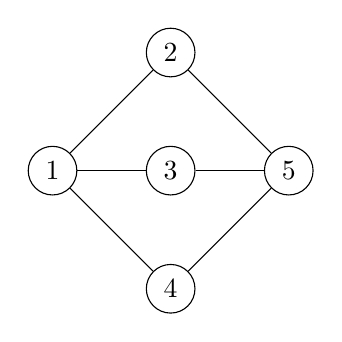
\begin{tikzpicture}[node distance={15mm}, main/.style = {draw, circle}] 
     \node[main] (1) {$1$};  
     \node[main] (3) [right of=1] {$3$};
     \node[main] (2) [above of=3] {$2$};
     \node[main] (4) [below of=3] {$4$};
     \node[main] (5) [right of=3] {$5$};

     \draw (1) -- (3);
     \draw (1) -- (2);
     \draw (1) -- (4);
     \draw (5) -- (2);
     \draw (5) -- (3);
     \draw (5) -- (4);
    \end{tikzpicture}
    \caption{Orbita pierwsza: 1, 5 
    Orbita druga: 2, 3, 4}
 \end{figure}


    \subsection{Kolorowanie grafu}
    \begin{definition}
      Dla grafu G = (V, E), wierzchołkowym oznakowaniem grafu nazywamy funkcję
       mapującą wierchołki do oznaczeń. Analogicznie, funkcję mapującą krawędzie do oznaczeń 
       nazywamy krawędziowym oznakowaniem grafu.  
    \end{definition}


    \begin{figure}[H]
      \centering
       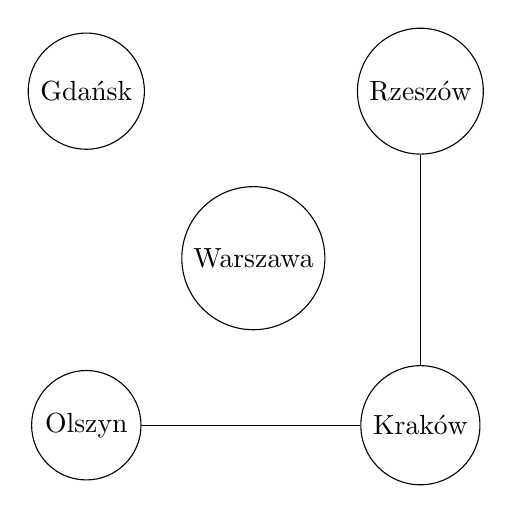
\begin{tikzpicture}[node distance={30mm}, main/.style = {draw, circle}] 
         \node[main] (1) {Gdańsk};
         \node[main] (3) [below right of=1] {Warszawa};
         \node[main] (2) [below left of=3] {Olszyn};
         \node[main] (4) [below right of=3] {Kraków};
         \node[main] (5) [above right of=3] {Rzeszów};

         \draw (2) -- (4);
         \draw (4) -- (5);

        \end{tikzpicture}
        \caption{ Przykład wierzchołkowego oznakowania grafu G z rysunku }
     \end{figure}

     \begin{figure}[H]
      \centering
       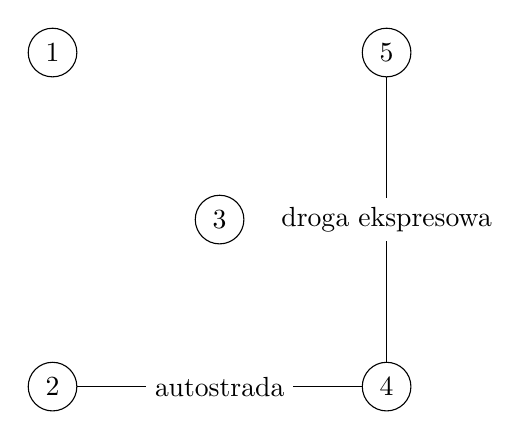
\begin{tikzpicture}[node distance={30mm}, main/.style = {draw, circle}] 
         \node[main] (1) {$1$};
         \node[main] (3) [below right of=1] {$3$};
         \node[main] (2) [below left of=3] {$2$};
         \node[main] (4) [below right of=3] {$4$};
         \node[main] (5) [above right of=3] {$5$};

         \draw (2) -- (4) node [midway, fill=white] {autostrada};
         \draw (4) -- (5) node [midway, fill=white] {droga ekspresowa};

        \end{tikzpicture}
        \caption{ Przykład krawędziowego oznakowania grafu G }
     \end{figure}

     Oznakowywanie elementów grafów ma wiele zastosowań. Często nadaje się krawędziom wartości, mające reprezentować, np.
     koszt pokonania drogi między dwoma punktami. Innym często wykorzystywanym oznakowaniem grafów jest kolorowanie.   
   
    \begin{definition}
      Kolorowanie grafów jest szczególnym przypadkiem oznakowywania grafu,
       w którym oznaczenia są nazywane kolorami i mogą być przypisywane tylko zgodnie z określonymi o
       ogranczeniami. 
    \end{definition}

    \begin{figure}[H]
      \centering
       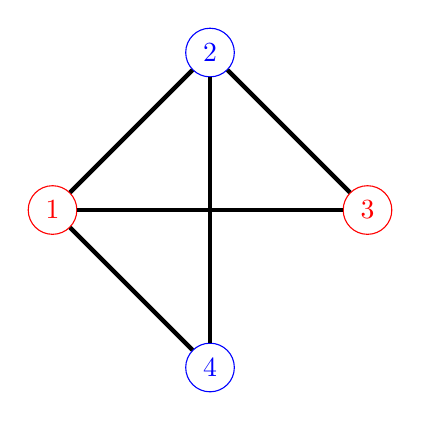
\begin{tikzpicture}[node distance={15mm}, main/.style = {draw, circle}] 
     \node[main][red] (3) at (0:2) {$3$};
     \node[main][blue] (2) at (90:2) {$2$};
     \node[main][red] (1) at (180:2) {$1$};
     \node[main][blue] (4) at (270:2) {$4$};
    
    \draw[ultra thick] (4) -- (1);
    \draw[ultra thick] (3) -- (2);
    \draw[ultra thick] (1) -- (3);

    \draw[ultra thick] (2) -- (1);
    \draw[ultra thick] (2) -- (4);
    \draw[ultra thick] (1) -- (3);
        \end{tikzpicture}
        \caption{Przykładowe kolorowanie wierzchołkowe grafu}
     \end{figure}

    \begin{figure}[H]
      \centering
       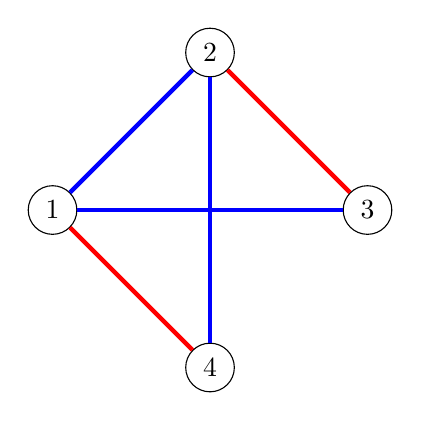
\begin{tikzpicture}[node distance={15mm}, main/.style = {draw, circle}] 
     \node[main] (3) at (0:2) {$3$};
     \node[main] (2) at (90:2) {$2$};
     \node[main] (1) at (180:2) {$1$};
     \node[main] (4) at (270:2) {$4$};
    
    \draw[ultra thick][red] (4) -- (1);
    \draw[ultra thick][red] (3) -- (2);
    \draw[ultra thick][red] (1) -- (3);
    
    
    \draw[ultra thick][blue] (2) -- (1);
    \draw[ultra thick][blue] (2) -- (4);
    \draw[ultra thick][blue] (1) -- (3);
        \end{tikzpicture}
        \caption{Przykładowe kolorowanie krawędziowe grafu}
     \end{figure}

     Kolorowanie najczęściej idzie w parze z ograniczeniami, których należy przestrzegać przypisując elementom wartości.
     Najczęściej dotyczą one zakazu kolorowania sąsiadujących wierzchołków lub krawędzi tym samym kolorem. 

     Innym ograniczeniem dla kolorowania może być zakaz pomalowania kliki ustalonego stopnia n - $K_n$ - tym samym kolorem.
     Dla $n=2$ otrzymamy zakaz sąsiedztwa wspomniany wcześniej.  